\documentclass[tikz,border=5pt]{standalone}
\usepackage{fix-cm}
% v3: data-led scientific illustration grammar. No dashboard cards or banners.
\usepackage{fix-cm}
\usepackage{amsmath,amssymb,graphicx}
\usepackage{tikz}
\usetikzlibrary{positioning,calc,fit,backgrounds,patterns,decorations.pathreplacing}
\renewcommand{\familydefault}{\sfdefault}
\definecolor{Ink}{HTML}{203848}
\definecolor{Muted}{HTML}{657884}
\definecolor{Rule}{HTML}{D2DDE3}
\definecolor{Observed}{HTML}{4E7897}
\definecolor{Teal}{HTML}{318E83}
\definecolor{Orange}{HTML}{C98542}
\definecolor{PaleBlue}{HTML}{EAF1F6}
\definecolor{PaleTeal}{HTML}{E8F3F0}
\definecolor{PaleOrange}{HTML}{FBF1E7}
\definecolor{GrayFill}{HTML}{F1F4F6}
\newcommand{\figfont}{\sffamily\fontsize{9.5}{11.5}\selectfont}
\newcommand{\figsmall}{\sffamily\fontsize{9}{10.5}\selectfont}
\tikzset{
 every node/.style={font=\figfont,text=Ink,inner sep=2pt},
 label/.style={font=\figfont,align=center},
 small/.style={font=\figsmall,text=Muted,align=center},
 panelletter/.style={font=\sffamily\bfseries\fontsize{10}{12}\selectfont,anchor=west},
 operator/.style={draw=Rule,fill=white,line width=.65pt,minimum height=.55cm,align=center,inner sep=4pt},
 flow/.style={->,>=stealth,draw=Ink!85,line width=.75pt},
 weight/.style={->,>=stealth,draw=Muted,dashed,line width=.65pt},
 axis/.style={->,>=stealth,draw=Muted,line width=.5pt},
 hair/.style={draw=Rule,line width=.5pt},
 sum/.style={circle,draw=Ink,fill=white,line width=.65pt,minimum size=12pt,inner sep=0pt},
}
% Illustrative 4x5 target table, not learned weights or experimental measurements.
% State 0: missing white; 1: initializer gray; 2: missing values restored in teal.
% Coordinates span [0,1.55] x [0,1.24]. No Other column is implied in this glyph.
\newcommand{\DataGrid}[1]{%
 \foreach \r in {0,...,3}{\foreach \c in {0,...,4}{%
  \pgfmathtruncatemacro{\tone}{25+mod(\r*17+\c*23,55)}
  \pgfmathtruncatemacro{\miss}{(\r==0&&\c==3)||(\r==1&&\c==0)||(\r==2&&\c==2)}
  \ifnum\miss=1
   \ifnum#1=0 \fill[white] (\c*.31,\r*.31) rectangle ++(.31,.31);
   \else\ifnum#1=1 \fill[Muted!22] (\c*.31,\r*.31) rectangle ++(.31,.31);
   \else \fill[Teal!65] (\c*.31,\r*.31) rectangle ++(.31,.31);\fi\fi
  \else \fill[Observed!\tone] (\c*.31,\r*.31) rectangle ++(.31,.31);\fi
  \draw[white,line width=.7pt] (\c*.31,\r*.31) rectangle ++(.31,.31);
 }}
 \draw[draw=Rule,line width=.55pt] (0,0) rectangle (1.55,1.24);
}
% A C-channel token is shown as a compact stack of editable vector strips.
\newcommand{\ChannelStrip}[1]{%
 \foreach \j in {0,...,7}{\pgfmathtruncatemacro{\tone}{25+mod(\j*17,55)}
  \fill[#1!\tone] (\j*.12,0) rectangle ++(.10,.43);}
}
\newcommand{\MaskGrid}{%
 \foreach \r in {0,...,3}{\foreach \c in {0,...,4}{%
  \pgfmathtruncatemacro{\miss}{(\r==0&&\c==3)||(\r==1&&\c==0)||(\r==2&&\c==2)}
  \ifnum\miss=1 \fill[white] (\c*.31,\r*.31) rectangle ++(.31,.31);
  \else \fill[Observed!55] (\c*.31,\r*.31) rectangle ++(.31,.31);\fi
  \draw[white,line width=.7pt] (\c*.31,\r*.31) rectangle ++(.31,.31);}}
 \draw[draw=Rule,line width=.55pt] (0,0) rectangle (1.55,1.24);
}
% Four parts x three real visits plus one padded row. Arrows identify axes,
% not numerical/learned attention weights. Mode 0 temporal; mode 1 feature.
\newcommand{\AxisGrid}[1]{%
 \fill[PaleBlue] (0,0) rectangle (1.28,1.28);
 \ifnum#1=0 \fill[Observed!22] (.32,.32) rectangle (.64,1.28);
 \else \fill[Teal!23] (0,.64) rectangle (1.28,.96);\fi
 \fill[GrayFill] (0,0) rectangle (1.28,.32);
 \foreach \i in {0,...,4}{
  \draw[draw=white,line width=.75pt] (\i*.32,0) -- (\i*.32,1.28);
  \draw[draw=white,line width=.75pt] (0,\i*.32) -- (1.28,\i*.32);}
 \draw[draw=Rule,line width=.5pt] (0,0) rectangle (1.28,1.28);
 \ifnum#1=0
  \draw[<->,>=stealth,draw=Observed,line width=1pt] (.48,.44) -- (.48,1.16);
 \else
  \draw[<->,>=stealth,draw=Teal,line width=1pt] (.12,.80) -- (1.16,.80);\fi
}

% Same cell coordinates in both views and all three stages.
% #1: 0 training, 1 inference. #2: 0 visible, 1 completion, 2 restored.
% Natural missing: (r,c)=(0,3),(1,0); H=(2,2); Q=(0,1),(3,4).
% Hatched Q locations contain NO truth values in the visible training matrix.
\newcommand{\ViewGrid}[2]{%
  \foreach \r in {0,...,3}{\foreach \c in {0,...,4}{%
    \pgfmathtruncatemacro{\tone}{25+mod(\r*17+\c*23,55)}
    \pgfmathtruncatemacro{\isq}{(\r==0&&\c==1)||(\r==3&&\c==4)}
    \pgfmathtruncatemacro{\ish}{\r==2&&\c==2}
    \pgfmathtruncatemacro{\hole}{(\r==0&&\c==3)||(\r==1&&\c==0)||\ish||(#1==0&&\isq)}
    \ifnum\hole=1
      \ifnum#2=0 \fill[white] (\c*.31,\r*.31) rectangle ++(.31,.31);
      \else\ifnum#2=1 \fill[Muted!22] (\c*.31,\r*.31) rectangle ++(.31,.31);
      \else \fill[Teal!65] (\c*.31,\r*.31) rectangle ++(.31,.31);\fi\fi
    \else \fill[Observed!\tone] (\c*.31,\r*.31) rectangle ++(.31,.31);\fi
    \draw[white,line width=.7pt] (\c*.31,\r*.31) rectangle ++(.31,.31);
    \ifnum#1=0 \ifnum\isq=1
      \ifnum#2=0
        \path[pattern=north east lines,pattern color=Orange!70]
          (\c*.31+.025,\r*.31+.025) rectangle ++(.26,.26);
      \fi
      \draw[Orange,line width=.65pt]
        (\c*.31+.025,\r*.31+.025) rectangle ++(.26,.26);
    \fi\fi
  }}
  \draw[Rule,line width=.55pt] (0,0) rectangle (1.55,1.24);
}
\begin{document}
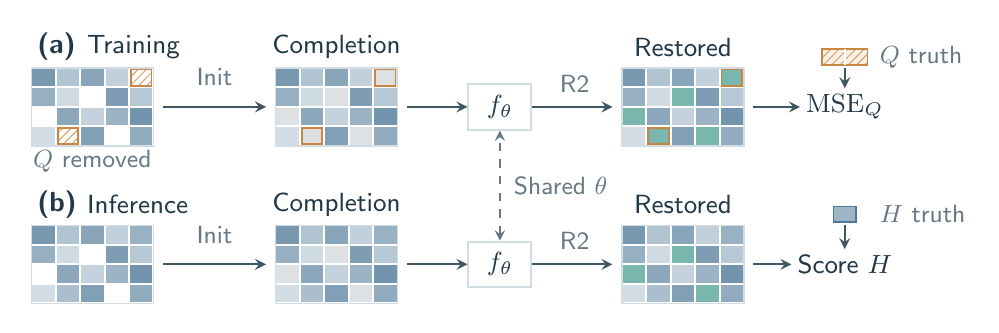
\begin{tikzpicture}[y=.8cm]
  \node[panelletter] at (0,4.22) {(a)};
  \node[label,anchor=west] at (.63,4.22) {Training};
  \node[label] at (3.875,4.22) {Completion};
  \node[label] at (8.275,4.22) {Restored};
  \begin{scope}[shift={(0,2.65)}]\ViewGrid{0}{0}\end{scope}
  \node[small] at (.775,2.40) {$Q$ removed};
  \begin{scope}[shift={(3.10,2.65)}]\ViewGrid{0}{1}\end{scope}
  \node[operator,minimum width=.80cm] (ft) at (5.95,3.27) {$f_\theta$};
  \begin{scope}[shift={(7.50,2.65)}]\ViewGrid{0}{2}\end{scope}
  \node[label] (loss) at (10.33,3.27) {$\mathrm{MSE}_Q$};

  \draw[flow] (1.67,3.27) -- (2.98,3.27);
  \node[small] at (2.325,3.74) {Init};
  \draw[flow] (4.77,3.27) -- (ft.west);
  \draw[flow] (ft.east) -- (7.38,3.27);
  \node[small] at (6.90,3.64) {R2};
  \draw[flow] (9.17,3.27) -- (loss.west);

  % Q labels have exactly one destination: the training loss.
  \fill[PaleOrange] (10.04,3.94) rectangle (10.62,4.19);
  \path[pattern=north east lines,pattern color=Orange!70]
    (10.04,3.94) rectangle (10.62,4.19);
  \draw[Orange,line width=.6pt] (10.04,3.94) rectangle (10.62,4.19);
  \draw[white,line width=.7pt] (10.33,3.94) -- (10.33,4.19);
  \node[small,anchor=west] at (10.70,4.065) {$Q$ truth};
  \draw[flow] (10.33,3.89) -- (loss.north);

  \node[panelletter] at (0,1.72) {(b)};
  \node[label,anchor=west] at (.63,1.72) {Inference};
  \node[label] at (3.875,1.72) {Completion};
  \node[label] at (8.275,1.72) {Restored};
  \begin{scope}[shift={(0,.15)}]\ViewGrid{1}{0}\end{scope}
  \begin{scope}[shift={(3.10,.15)}]\ViewGrid{1}{1}\end{scope}
  \node[operator,minimum width=.80cm] (fi) at (5.95,.77) {$f_\theta$};
  \begin{scope}[shift={(7.50,.15)}]\ViewGrid{1}{2}\end{scope}
  \node[label] (score) at (10.33,.77) {Score $H$};

  \draw[flow] (1.67,.77) -- (2.98,.77);
  \node[small] at (2.325,1.24) {Init};
  \draw[flow] (4.77,.77) -- (fi.west);
  \draw[flow] (fi.east) -- (7.38,.77);
  \node[small] at (6.90,1.14) {R2};
  \draw[flow] (9.17,.77) -- (score.west);

  % H labels have exactly one destination: held-out scoring.
  \fill[Observed!55] (10.185,1.44) rectangle (10.475,1.69);
  \draw[Observed,line width=.6pt] (10.185,1.44) rectangle (10.475,1.69);
  \node[small,anchor=west] at (10.70,1.565) {$H$ truth};
  \draw[flow] (10.33,1.39) -- (score.north);

  % Only the parameters are paired; completed data never cross between lanes.
  \draw[weight,<->] (fi.north) -- (ft.south);
  \node[small,anchor=west,fill=white] at (6.05,2.02) {Shared $\theta$};

\end{tikzpicture}
\end{document}
